\chapter{Design architetturale}

Di seguito viene raffigurata la struttura del sistema che si realizzerà successivamente in fase di tesi.

\begin{figure}[H]
\centering
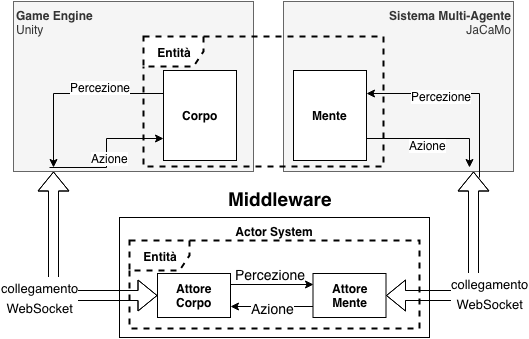
\includegraphics[width=\textwidth]{figures/Synapsis.png}
\caption{Design architetturale}
\end{figure}

Dallo schema è possibile notare come vengono utilizzate le tecnologie precedentemente illustrate:
\begin{itemize}
    \item La Game Engine Unity è adatta ad ospitare il corpo di una generica entità;
    \item JaCaMo è adatto ad ospitare la mente di una generica entità;
    \item Il framework Play viene utilizzato per realizzare il middleware che collega i due sistemi;
    \item La reale connessione viene creata attraverso il protocollo WebSocket integrabile a JaCaMo, Unity e nativamente supportato nel framework Play.
\end{itemize}

Questa soluzione permette a mente e corpo di scambiarsi informazioni, anche se computazionalmente risiedono in sistemi separati, lasciando intatte funzionalità e astrazioni presenti nel Sistema Multi-Agente e nella Game Engine.

\medskip

Con Unity viene "fisicamente" realizzato il corpo di una generica entità: utilizzando il concetto di GameObject ed attraverso i componenti, quali Collidere, Rigibody e script contenenti il collegamento WebSocket, è possibile dotare il corpo di funzionalità adatte a percepire l'ambiente. Ad esempio, in caso di contatto/urto con un diverso oggetto in scena, esso è capace di avvertire l'evento ed inviare alla mente una percezione del tipo \textit{"toccato(nome\_entità\_toccata)"}. 

\medskip

Attraverso Jason viene realizzata la mente dell'entità utilizzando il concetto di agente unito ad un artefatto. Ciò permette di rappresentare il corpo dell'entità all'interno del MAS, interfacciandosi alla GE tramite l'artefatto che contiene la connessione WebSocket. Ad esempio, se la mente vuole far eseguire al corpo una determinata azione è sufficiente che utilizzi l'artefatto collegato per inviare un'azione del tipo \textit{vai\_a (posizione)};

\section{Scenario d'esempio}

Per meglio comprendere l'architettura di sistema appena descritta, e le interazioni tra i suoi componenti costituenti, si prende a riferimento uno scenario d'esempio chiamato "recycling robots". Come si può intuire dal nome, la scena contiene dei robot, i quali hanno il compito di riciclare la spazzatura presente nell'ambiente portandola in un bidone.

\medskip

Il compito generale di un robot è divisibile in un ciclo di sotto-obiettivi, ad esempio:
\begin{enumerate}
    \item Cercare la spazzatura;
    \item Andare verso la spazzatura trovata;
    \item Prendere la spazzatura appena raggiunta;
    \item Cercare il bidone
    \item Andare verso il bidone trovato
    \item Riciclare la spazzatura
\end{enumerate}

Utilizzando il formalismo di Jason, i sotto-obiettivi elencati sono associabili a dei \textit{"plans"} di un agente. Al di fuori del primo plan (Cercare la spazzatura), normalmente attivato dal \textit{"goal"} principale presente nell'agente, i successivi possono essere attivati da una percezione ricevuta dall'agente. Ad esempio, in risposta alla ricerca del bidone è possibile notificare la scoperta di un bidone nelle vicinanze e, di conseguenza, fare in modo che l'agente utilizzi il plan "Andare verso il bidone trovato".

\begin{figure}[H]
\centering
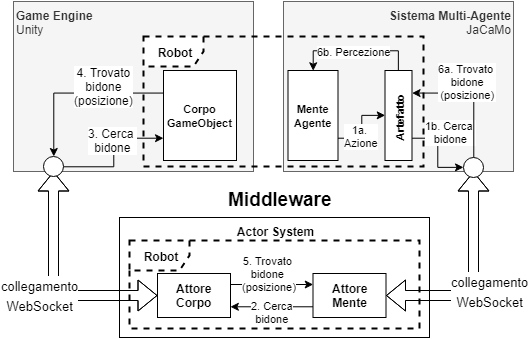
\includegraphics[width=0.7\textwidth]{figures/Esempio.png}
\caption{Esempio di comunicazione tra mente e corpo}
\end{figure}

L'immagine mostra il flusso ordinato di interazioni atteso per l'esempio appena descritto. La mente per svolgere il plan \textit{"Cercare il bidone"} vuole inviare al proprio corpo l'azione \textit{"Cerca bidone"}. Il trasferimento del messaggio avviene attraverso l'artefatto personale dell'agente\footnote{previa associazione dei due}, in possesso del canale WebSocket collegato al middleware, dove è presente un'operazione che invia il messaggio al middleware.

\medskip 

L'attore mente presente nel middleware alla ricezione delle infomazioni da inviare al corpo, inoltra le stesse all'attore corpo che è l'unico possessore del riferimento all'entità corpo presente su Unity e, quindi, in grado di inoltrare il messaggio al corpo "reale". Quando su Unity l'entità corpo (GameObject) riceve il messaggio, attraverso il canale WebSocket, attua l'azione a lui richiesta e risponde alla mente inviando la percezione generata.

\medskip

A questo punto la percezione viene mandata al middleware, più precisamente all'attore "corpo" che a sua volta la inoltrerà all'attore "mente", che la invierà poi all'artefatto collegato, sempre tramite WebSocket.

\medskip

L'artefatto, alla ricezione della percezione, aggiunge quest'ultima alle sue proprietà osservabili che, automaticamente, aggiorneranno la BeliefBase dell'agente. L'ultimo passaggio rappresenta il punto cruciale per completare il collegamento tra corpo e mente dato che in questa maniera l'agente ha ricevuto la percezione dal proprio corpo. 

\medskip

Si intende inoltre lasciare aperta la possibilità, da parte del corpo, di inviare percezioni non come reazione ad azioni eseguite dalla mente, dato che il collegamento WebSocket, una volta effettuato, rimane attivo per tutta la durata di vita dell'entità. Ad esempio, in caso di contatto con un oggetto nella scena Unity, il corpo deve essere in grado di mandare una percezione del tipo \textit{"toccata(nome\_oggetto,posizione)"} alla propria mente senza bisogno di stimoli.

\medskip

Per concludere, il lavoro di attività propedeutica ha permesso di acquisire la necessaria conoscenza e dimestichezza con i concetti e le tecnologie da utilizzare per la successiva realizzazione del middleware in fase di tesi.
 